\chapter{La mesure et sa représentation}
\label{chap:measurements}

Lors de tout procédé expérimental, on effectue des mesures. Une mesure brute, seule, ne veut presque rien dire (éventuellement on obtient l'ordre de grandeur). Il faut lui adjoindre une estimation d'incertitude. La plupart du temps, lorsque l'on a besoin d'une connaissance précise des caractéristiques d'un système quelconque, on va réaliser un grand nombre de mesures individuelles de ces propriétés, et c'est l'analyse statistique des mesures qui va nous permettre d'estimer les propriétés du système, avec marge d'incertitude. Cette démarche en deux temps, (1) acquisition d'un nombre significatif de données (2) traitement statistique de ces données, constitue le c\oe ur de la démarche expérimentale. Elle seule permet d'obtenir des résultats valides.

Avant d'appliquer les outils de l'analyse statistique à un échantillon de mesures, il est cependant indispensable d'examiner \textbf{la qualité de l'échantillon}: existe-t-il des valeurs aberrantes qu'il faudrait rejeter ? Y a-t-il assez de mesures ? etc. On utilise pour cela des outils de représentation simples: moyenne, écart-type, et surtout, l'histogramme. Ce chapitre est donc dédié à la définition de ce que c'est qu'une mesure, et des outils permettant de la valider, et de la caractériser.

\section{Définitions}

\subsection{L'échantillon}

Soit une grandeur physique $\mathcal{G}$ (par exemple une tension électrique) et un ensemble de $N_m$ mesures de $\mathcal{G}$. Cet ensemble est appelé un \textbf{échantillon} $\mathcal{E}$ de $\mathcal{G}$. Quelques exemples:
\begin{description}
\item[mesures de la tension aux bornes d'une résistance] $\mathcal{E}=[3.5,3.4,3.1,3.7]$ mV,
\item[cinq jets d'un dé à 6 faces] $\mathcal{E}=[5,4,1,2,2]$,
\item[une séquence du génome humain] $\mathcal{E}=[A,G,G,T,A,G,G,T,C,C,A]$,
\item[mesure d'un diamètre d'axe] $\mathcal{E}=[19.998,20.004,20.003,19.997,20.013]$ mm.
\end{description}
On voit que les éléments d'un échantillon peuvent être de tout type, entier ou réel, et même non numérique. Ce qui caractérise un échantillon, c'est la \textbf{nature} et le \textbf{nombre} de ses éléments (quoi, et combien).

\subsection{La population}

La population $\mathcal{P}$ d'une grandeur $\mathcal{G}$ est définie par \textbf{l'ensemble de toutes les valeurs possibles que peut prendre cette grandeur}. C'est à partir de la population que l'on forme des échantillons. Quelques exemples:
\begin{description}
\item[dé à 6 faces] $\mathcal{P}=[1,2,3,4,5,6]$,
\item[les lettres du génome humain] $\mathcal{P}=[A,C,G,T]$
\item[mesure d'un diamètre de 20 mm] $\mathcal{P}=\infty$ !
\end{description}
Quelques remarques s'imposent:
\begin{itemize}
\item la longueur d'un échantillon peut être inférieure, égale ou supérieure à la dimension de la population: il s'agit simplement du nombre de mesures effectuées;
\item la dimension d'une population peut être infinie ! par exemple, dans le cas de la mesure du diamètre d'un axe, les fluctuations de la mesure dues à la précision toujours limitée de l'instrument de mesure, ou aux variations de la pièce elle-même (dilatation/contraction thermique), vont induire une mesure dont la différence avec la valeur réelle sera aléatoire.
\end{itemize}
Il n'est pas toujours évident de déterminer la population d'une mesure. Seule une inspection détaillée du processus de mesure nous permettra de déterminer au cas par cas la population complète de $\mathcal{G}$.

À quoi sert-il de déterminer la population ? Tout simplement à connaître à l'avance les résultats possibles des mesures, et éliminer par avance les mesures impossibles. Un exemple: admettons qu'un ingénieur ait mis au point un appareil automatique de mesure de diamètre, et que l'on soumette à cet appareil un axe cylindrique de 20 mm de diamètre. Quatre mesures sont effectuées, et l'échantillon est le suivant $\mathcal{E}=[19.9,20.1,1.7,19.8]$ mm. Immédiatement, on voit que la valeur des 3$^\text{ème}$ mesures n'a aucun sens, elle ne peut vraiment pas faire partie de la population. L'ingénieur en conclut qu'il y a un problème avec le procédé de mesure.

\subsection{L'analyse statistique}

L'analyse statistique \textit{est un ensemble de méthodes de traitement numérique d'un échantillon permettant d'estimer les propriétés de la population dont il est issu.}

Pour donner un exemple, imaginons que nous disposions d'un échantillon de mesure d'une tension électrique. Les outils de l'analyse statistique nous permettront de calculer l'incertitude sur la moyenne de l'échantillon, ce qui est une information aussi importante que la moyenne elle-même.

On peut aussi dire: \textit{l'analyse statistique permet de réduire un ensemble de données brutes en un petit nombre de valeurs caractéristiques de la population associée}. C'est assez identique à la première définition. On parle aussi de \textbf{réduction} des données.

\section{Moyenne, écart quadratique moyen, écart-type}

Soit un échantillon de $N_m$ mesures de la grandeur $\mathcal{G}$. Désignons par $x_i$ la valeur de la mesure individuelle numéro $i$, avec $i=1\dots N_m$.

\subsection{La moyenne de l'échantillon}

Elle est définie par
\begin{equation}
\langle x\rangle=\frac{1}{N_m}\sum\limits_{i=1}^{N_m}\,x_i
\end{equation}
Notation: les parenthèses angulaires $\langle\cdot\rangle$ désignent l'opération de moyenne. On rencontre aussi dans la littérature le symbole $\overline{x}$, mais la première notation est plus fréquente.

\subsection{L'écart quadratique moyen de l'échantillon}

C'est la moyenne de l'écart quadratique (c.-à-d. au carré) entre les éléments de l'échantillon et sa valeur moyenne $\langle x\rangle$,
\begin{equation}
\text{EQM}(x)=\langle (x-\langle x\rangle)^2\rangle
\end{equation}
Si nous développons, il vient
$$
\langle (x-\langle x\rangle)^2\rangle=\langle x^2-2x\langle x\rangle+\langle x\rangle^2\rangle
=\langle x^2\rangle-2\langle x\rangle\langle x\rangle+\langle\langle x\rangle^2\rangle
=\langle x^2\rangle-2\langle x\rangle^2+\langle x\rangle^2
=\langle x^2\rangle-\langle x\rangle^2
$$
d'où, en appliquant la définition de la moyenne
\begin{equation}
\text{EQM}(x)=\frac{1}{N_m}\sum\limits_{i=1}^{N_m}\,x_i^2-
\left(\frac{1}{N_m}\sum\limits_{i=1}^{N_m}\,x_i\right)^2
\end{equation}
À noter que l'on désigne aussi l'écart quadratique moyen par la \textbf{variance} de l'échantillon, mais comme ce dernier terme possède une définition très spécifique en relation avec les distributions de probabilité, il vaut mieux ne pas l'utiliser dans le contexte d'un échantillon de taille finie.

\subsection{L'écart-type de l'échantillon}

Il est simplement défini par la racine carrée de l'écart quadratique moyen, et on le note avec le symbole $\sigma$
\begin{equation}
\sigma(x)=\sqrt{\text{EQM}(x)}
\end{equation}
Il représente la \textbf{dispersion typique des mesures} autour de la moyenne.
\vspace{3mm}
\begin{center}
\fbox{
\begin{minipage}{12cm}\textbf{L'écart-type et la moyenne constituent les deux outils centraux de l'analyse statistique d'un échantillon.}
\end{minipage}
}
\end{center}

\section{La représentation d'un échantillon de mesures à l'aide d'un histogramme}

\begin{figure}[htb]
   \centering
   \vspace{-5mm}
   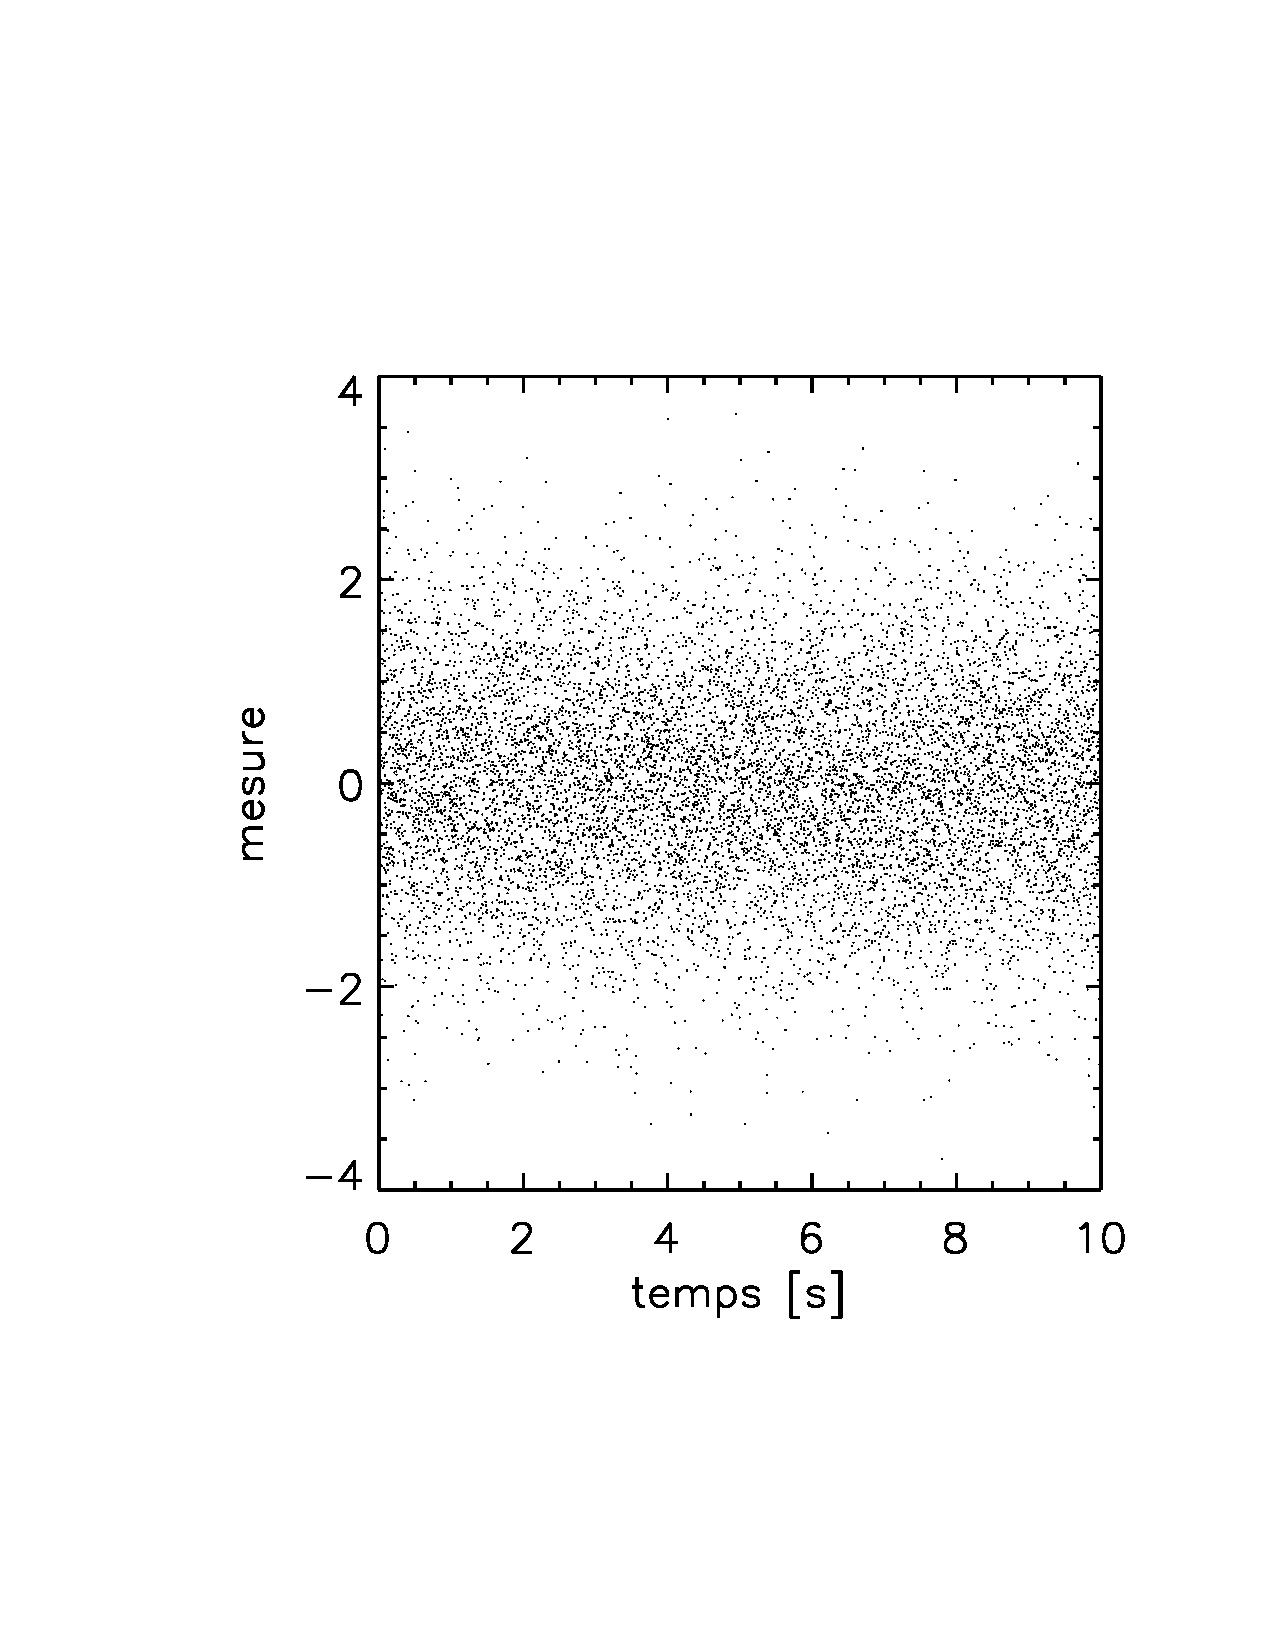
\includegraphics[width=6cm]{assets/figures/serie1000points.pdf} \hspace{5mm}
   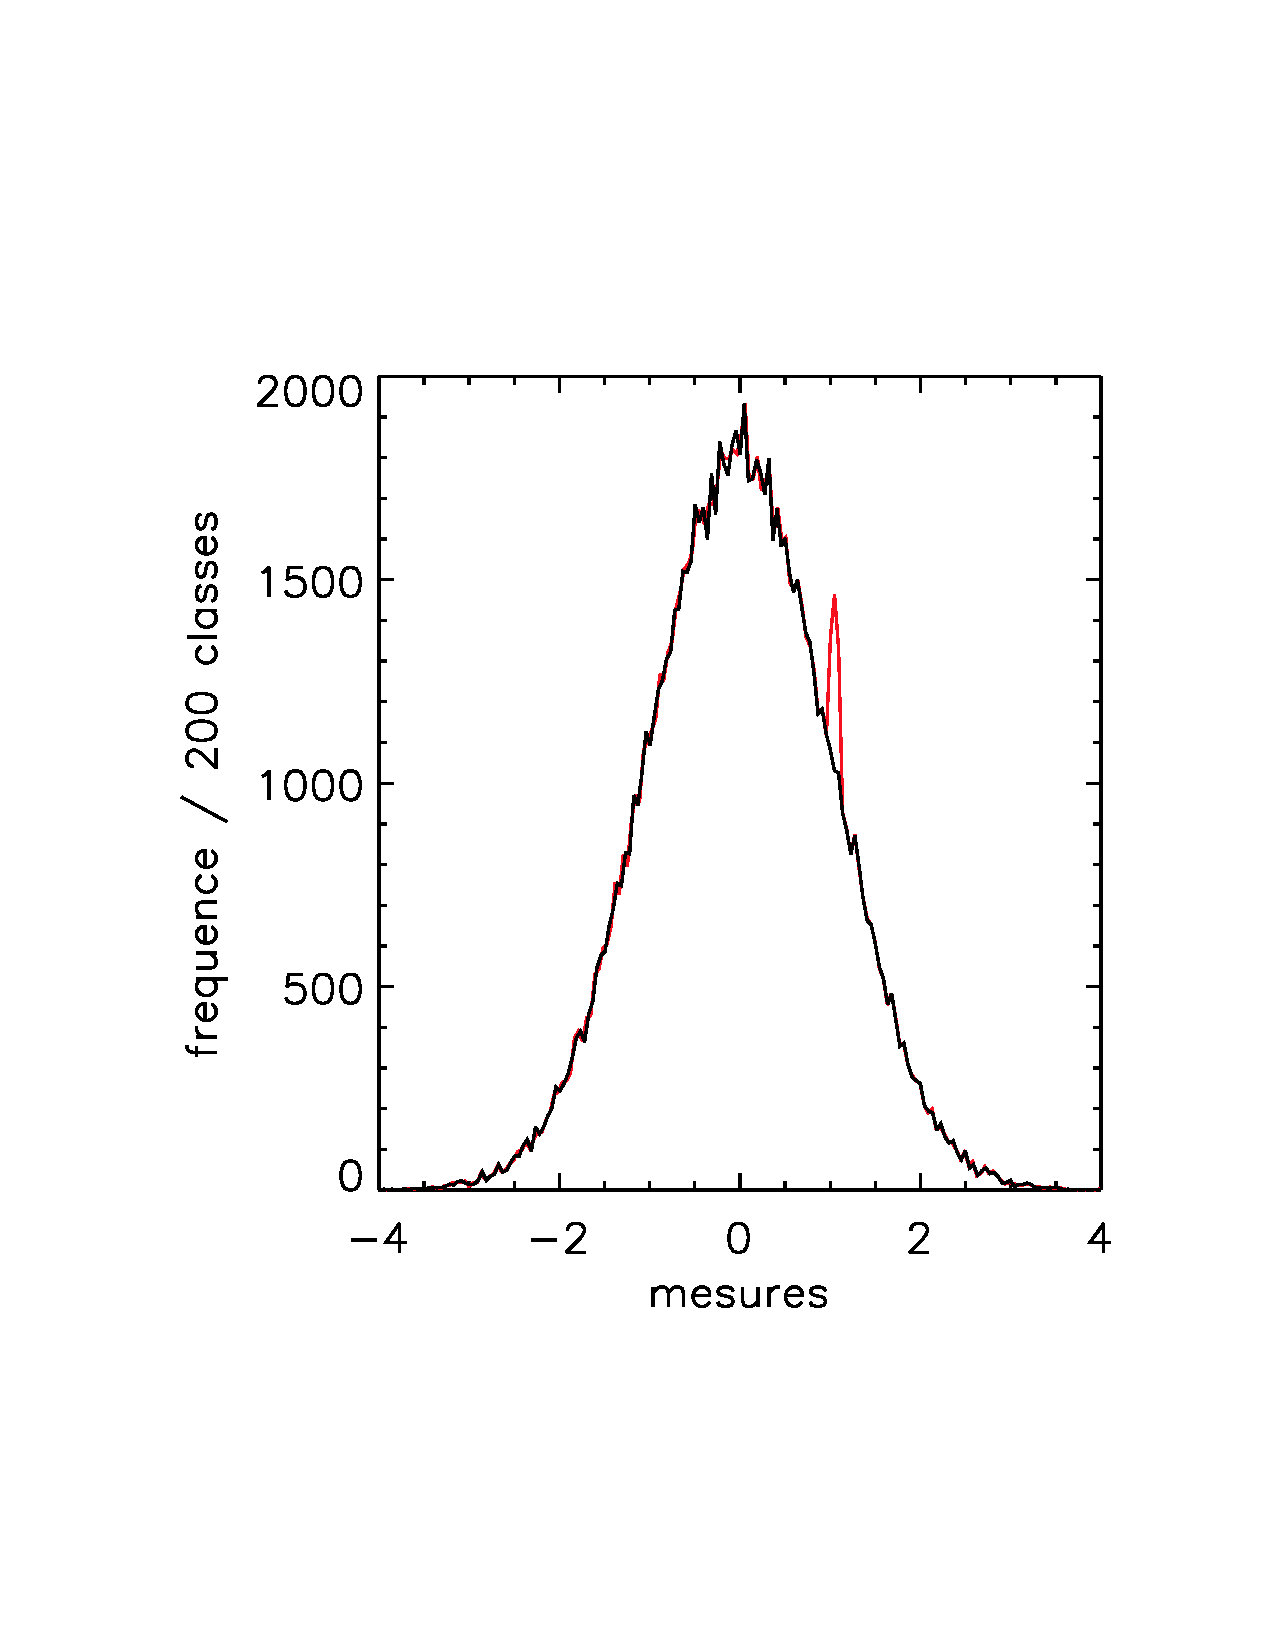
\includegraphics[width=6cm]{assets/figures/serie1000points_histogram.pdf}
   \caption{\it À gauche: les 1000 premières mesures d'une série de 100'000 mesures, pour lesquelles on sait qu'il existe une mesure parasite autour de la valeur 1. Elle est invisible dans ce graphique. À droite: histogramme des 100'000 mesures. En noir, histogramme sans le signal parasite. En rouge, histogramme avec le signal parasite.}
   \label{fig:sdp}
\end{figure}
En général, les échantillons de mesure sont constitués d'un grand nombre d'éléments - quelques dizaines lorsque l'acquisition se fait à la main, à plusieurs milliers ou plus lorsque l'acquisition se fait de manière automatique (ce qui est préférable).

Or, avant d'exploiter les données, il faut les examiner, afin de détecter un problème éventuel - ce qui arrive toujours lors de la phase de mise au point d'un instrument ou d'une machine. Il est donc crucial de \textbf{visualiser} les échantillons. Si la dimension de l'échantillon est grand, il peut être pratiquement impossible (ou peu pratique) d'examiner chaque mesure individuelle (figure~\ref{fig:sdp}). Dans ce cas, on utilisera avec avantage une représentation graphique, \textbf{l'histogramme}.

L'idée de l'histogramme consiste à segmenter l'intervalle entre la valeur minimale et la valeur maximale de l'échantillon en $N_c$ sous-intervalles - ou classes - de même largeur, puis à compter le nombre de fois que les mesures tombent dans chacune des classes. On établit alors un graphique montrant le nombre de mesures dans chaque classe, qui nous donne une vue d'ensemble immédiate, permettant de détecter la présence éventuelle de mesures problématiques, pour autant que nous ayons une idée préalable des valeurs que peuvent prendre les mesures (la population).

Considérons l'exemple de la figure~\ref{fig:sdp}. Il s'agit d'un échantillon de 100'000 mesures d'une grandeur physique (quelconque, dont on ne précise pas l'unité) de moyenne nulle, et d'écart-type $\sigma=1$. On montre la série des 1'000 premiers points de mesure. On a ajouté, à cette série de mesures, un \textbf{signal parasite} de moyenne égale à 1 et d'écart-type 0.1. Ce signal parasite n'est pas du tout visible parmi la série des 1'000 points de mesure. En revanche, l'histogramme montre très bien, centré sur 1, un excès du nombre de mesures (ou fréquence) par rapport à la fréquence des valeurs voisines.

\begin{figure}[h]
   \centering
   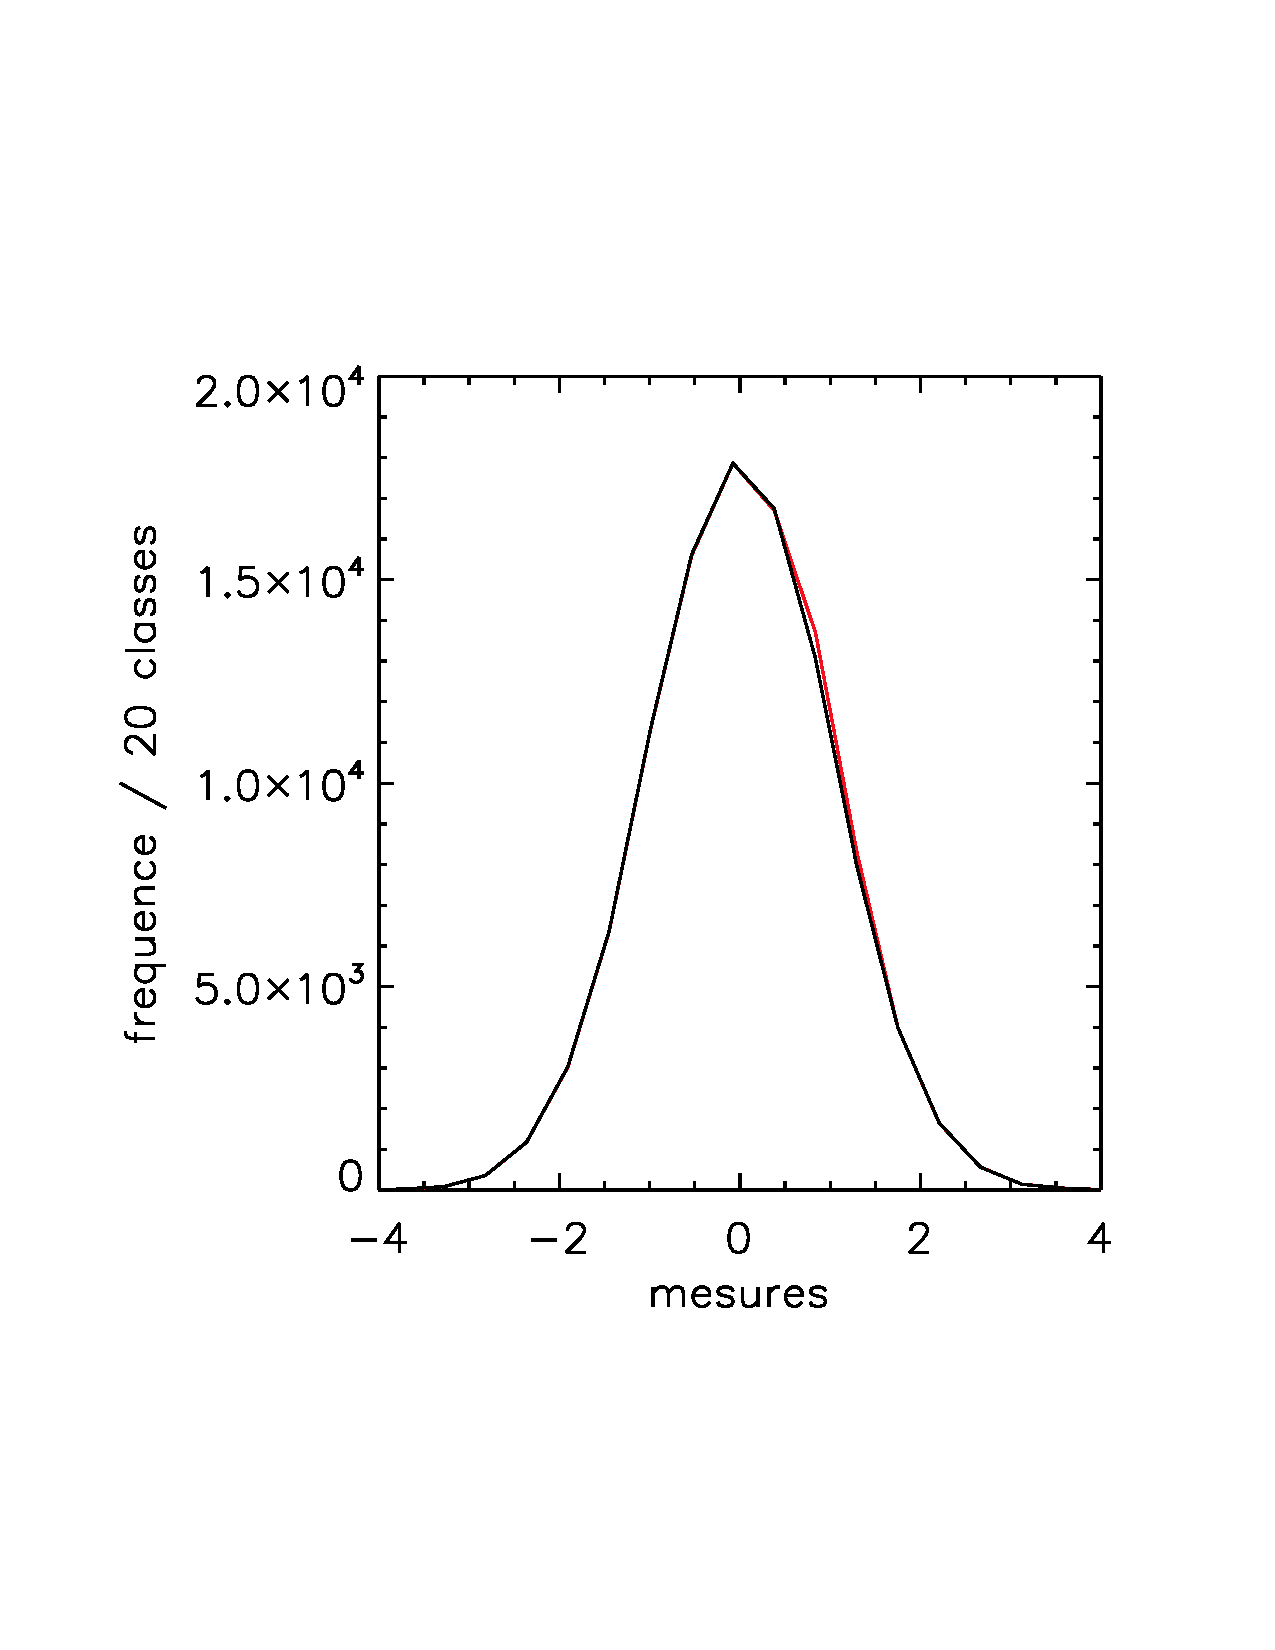
\includegraphics[height=6cm]{assets/figures/serie1000points_histogram_20classes.pdf} \hspace{5mm}
   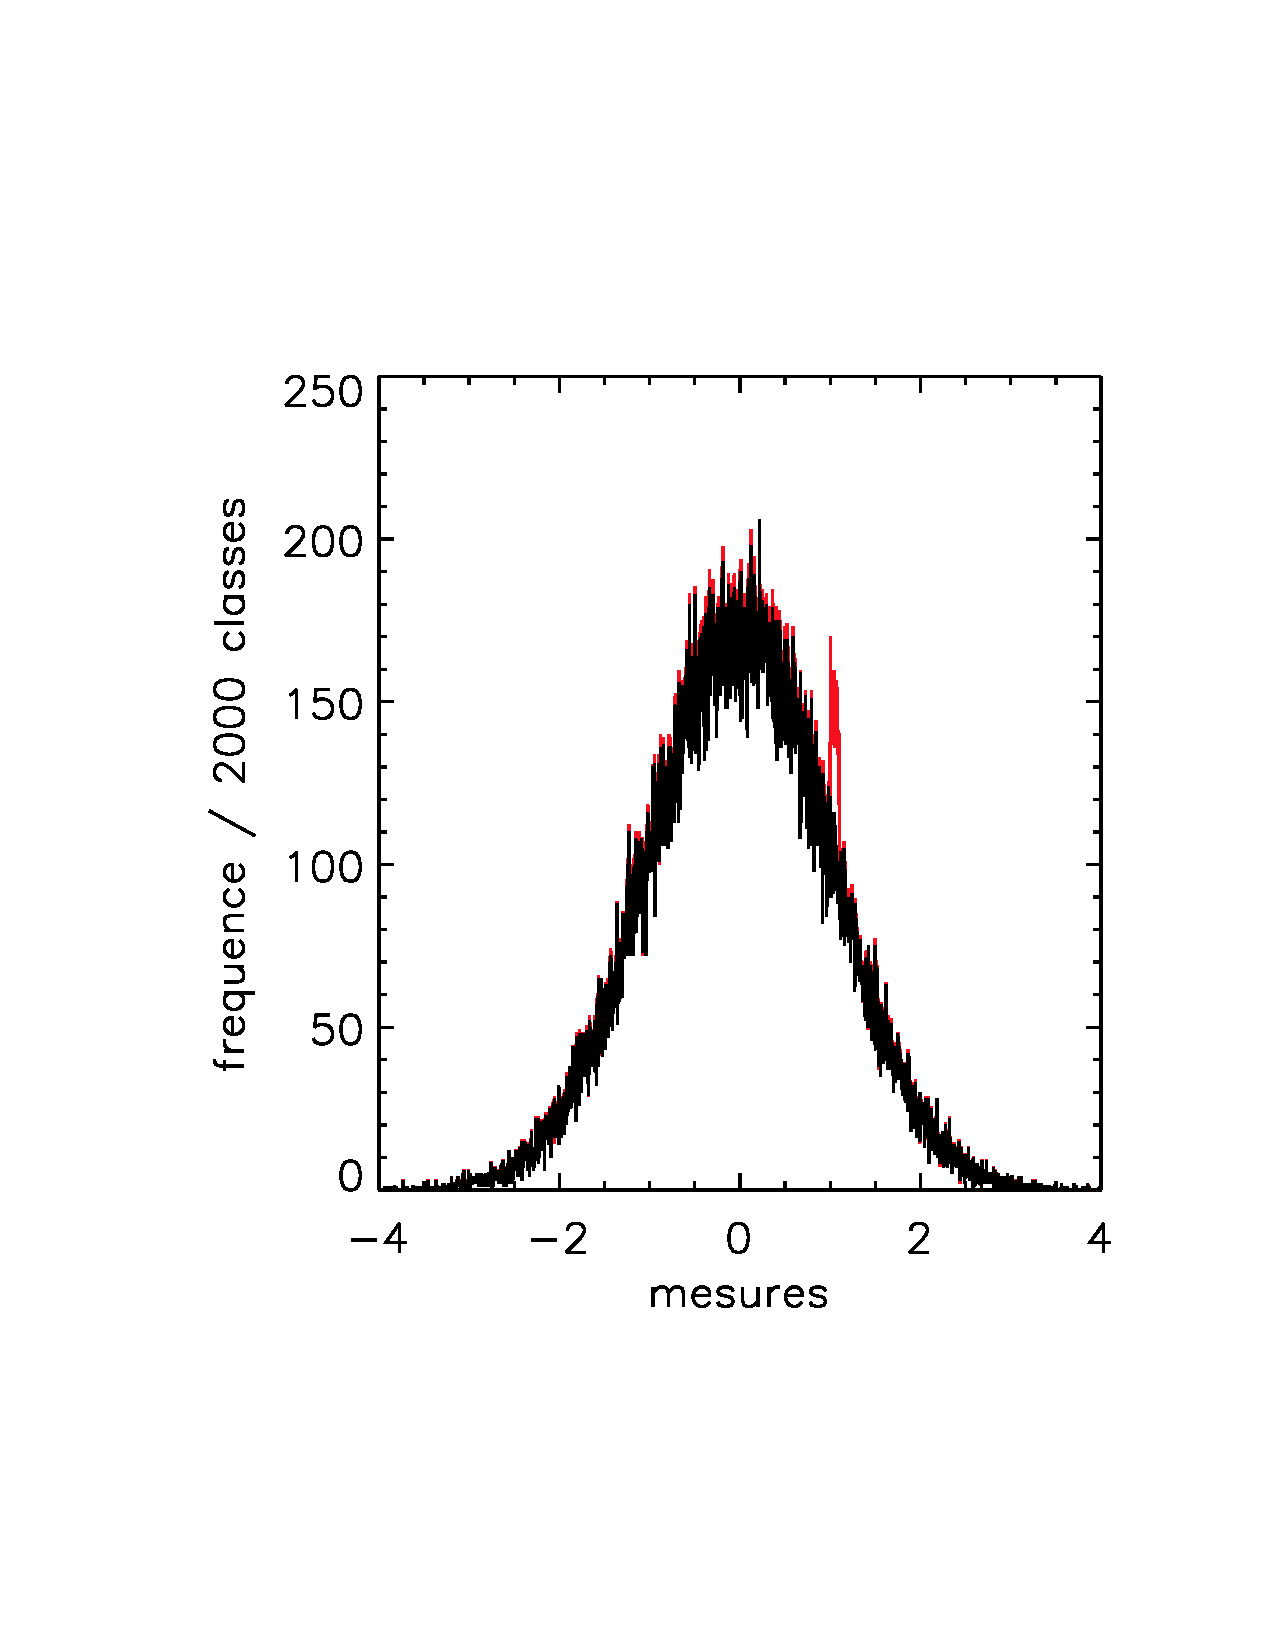
\includegraphics[height=6cm]{assets/figures/serie1000points_histogram_2000classes.pdf}
   \caption{Histogramme des 100'000 mesures, avec 20 classes, à gauche, et 2000 classes, à droite. En noir, histogramme du signal sans signal parasite. En rouge, histogramme du signal avec le signal parasite.}
   \label{fig:hapoabdc}
\end{figure}
Toute la difficulté consiste à choisir le nombre de classes. Dans l'exemple ci-dessus, nous avons considéré 200 classes. Si nous avions pris moins de classes, par exemple 20, alors l'histogramme serait plus lisse (figure~\ref{fig:hapoabdc}), mais la résolution trop grossière, et nous n'aurions pas détecté les mesures parasites. En revanche, avec beaucoup de classes (2000), la résolution est grande, mais l'histogramme devient plus chaotique, et il se pourrait que le signal parasite soit noyé dans les fluctuations statistiques (ce qui n'est en fait pas encore le cas ici).

Une bonne méthode empirique pour choisir le nombre de classes est de prendre la racine carrée du nombre de mesures. Pour 100'000, nous devrions prendre 316 classes. Quoi qu'il en soit, le nombre optimal de classes sera celui qui nous permettra de visualiser au mieux les propriétés de notre échantillon de mesures. On a vu que pour notre exemple, avec 200 classes on obtient en pratique une très bonne représentation.

\subsection{Comment interpréter un histogramme ?}

\begin{itemize}
\item si l'histogramme est symétrique, alors la valeur sur laquelle il est centré est une indication de la valeur moyenne de l'échantillon; s'il n'est pas symétrique, on ne peut rien dire sur la valeur moyenne, et il faut faire un calcul;
\item la valeur de la mesure correspondant au maximum de l'histogramme définit le \textbf{mode} de l'échantillon. C'est la valeur \textbf{la plus fréquente}. Qui se confond avec la valeur moyenne seulement si l'histogramme est symétrique;
\item la largeur à mi-hauteur de l'histogramme est une indication de la dispersion des mesures, et est directement reliée à l'écart-type $\sigma(x)$.
\item la forme de l'histogramme est une indication du type de processus statistique à l'\oe uvre lors de l'acquisition de l'échantillon (on aura des processus de type gaussien, poissonien, binomial, uniforme, etc - que l'on introduira plus loin). Or, il est possible de prévoir, pour un processus de mesure donné, le type de distribution attendu. La comparaison de la forme de l'histogramme des mesures avec la distribution prévue nous permettra de confirmer que le système se comporte de la manière attendue. Par exemple, le pic dans l'histogramme de l'exemple précédent dévoile l'existence du signal parasite, car en général, toutes les mesures de grandeurs physiques suivent des distributions régulières (ici une distribution dite gaussienne).
\end{itemize}

\subsection{La distribution gaussienne}

On discutera, dans le chapitre dédié aux distributions, de la répartition dite gaussienne d'une mesure aléatoire. Mais comme il s'agit d'une distribution très fréquemment utilisée en pratique, et que nous utilisons souvent comme référence, il est utile de l'introduire rapidement ici.

Dans la grande majorité des cas, lorsque l'on mesure la valeur d'une grandeur physique de type \textbf{réel}\footnote{c.-à-d. ne prenant pas des valeurs discrètes, mais pouvant avoir toute valeur dans l'intervalle des nombres réels} soumise à des fluctuations aléatoires, comme la tension électrique, la température, etc., on trouve que les mesures se répartissent symétriquement autour d'une moyenne, selon une courbe dite \textit{en cloche}. L'équation de cette répartition est la suivante
\begin{equation}
g(x)=\frac{1}{\sigma\sqrt{2\pi}}\exp{\left[-\frac{(x-\mu)^2}{2\sigma^2}\right]}
\end{equation}
ou $\mu$ représente la moyenne des mesures et $\sigma$ l'écart-type de la grandeur physique $x$. Les 100'000 points dont on a représenté l'histogramme à 20 classes en figure~\ref{fig:hapoabdc} suit une distribution gaussienne de moyenne $\mu=0$ et d'écart-type $\sigma=1$.

\subsection*{Histogramme, ou distribution de probabilité ? et combien de mesures faut-il acquérir ?}

Il y a une grande différence conceptuelle entre un histogramme et une distribution de probabilité. Un histogramme n'est qu'une représentation graphique des fréquences associées à \textbf{un seul échantillon} de mesures. En principe, si on enregistre N échantillons de mesures de la même grandeur physique, on va tomber sur N histogrammes légèrement différents les uns des autres car il n'y a aucune raison de mesurer à chaque fois la même série de valeurs !

En revanche, si on effectue une infinité de mesures ($N_m\rightarrow\infty$), alors la fréquence relative $p_k=f_k/N_m$ va tendre vers une valeur stable, constante, qui pourra s'interpréter comme la probabilité que la mesure tombe dans la classe $k$. On verra alors plus loin que dans ce cas, il peut y avoir égalité exacte entre les moyennes et EQM calculés à partir de l'échantillon ou à partir de la distribution des probabilités.

Il ressort de tout cela que si on désire avoir une bonne estimation de la structure de la distribution des valeurs, il faut considérer des échantillons de mesure assez grands.  Typiquement, une centaine de mesures permet déjà de se faire une idée de la répartition sous-jacente. Mais ce n'est qu'avec 1000 points que l'on arrive vraiment à identifier le type de distribution. La figure~\ref{fig:h123} montre l'évolution de l'histogramme associé à une \begin{wrapfigure}[19]{l}[0pt]{6cm}
   \centering
   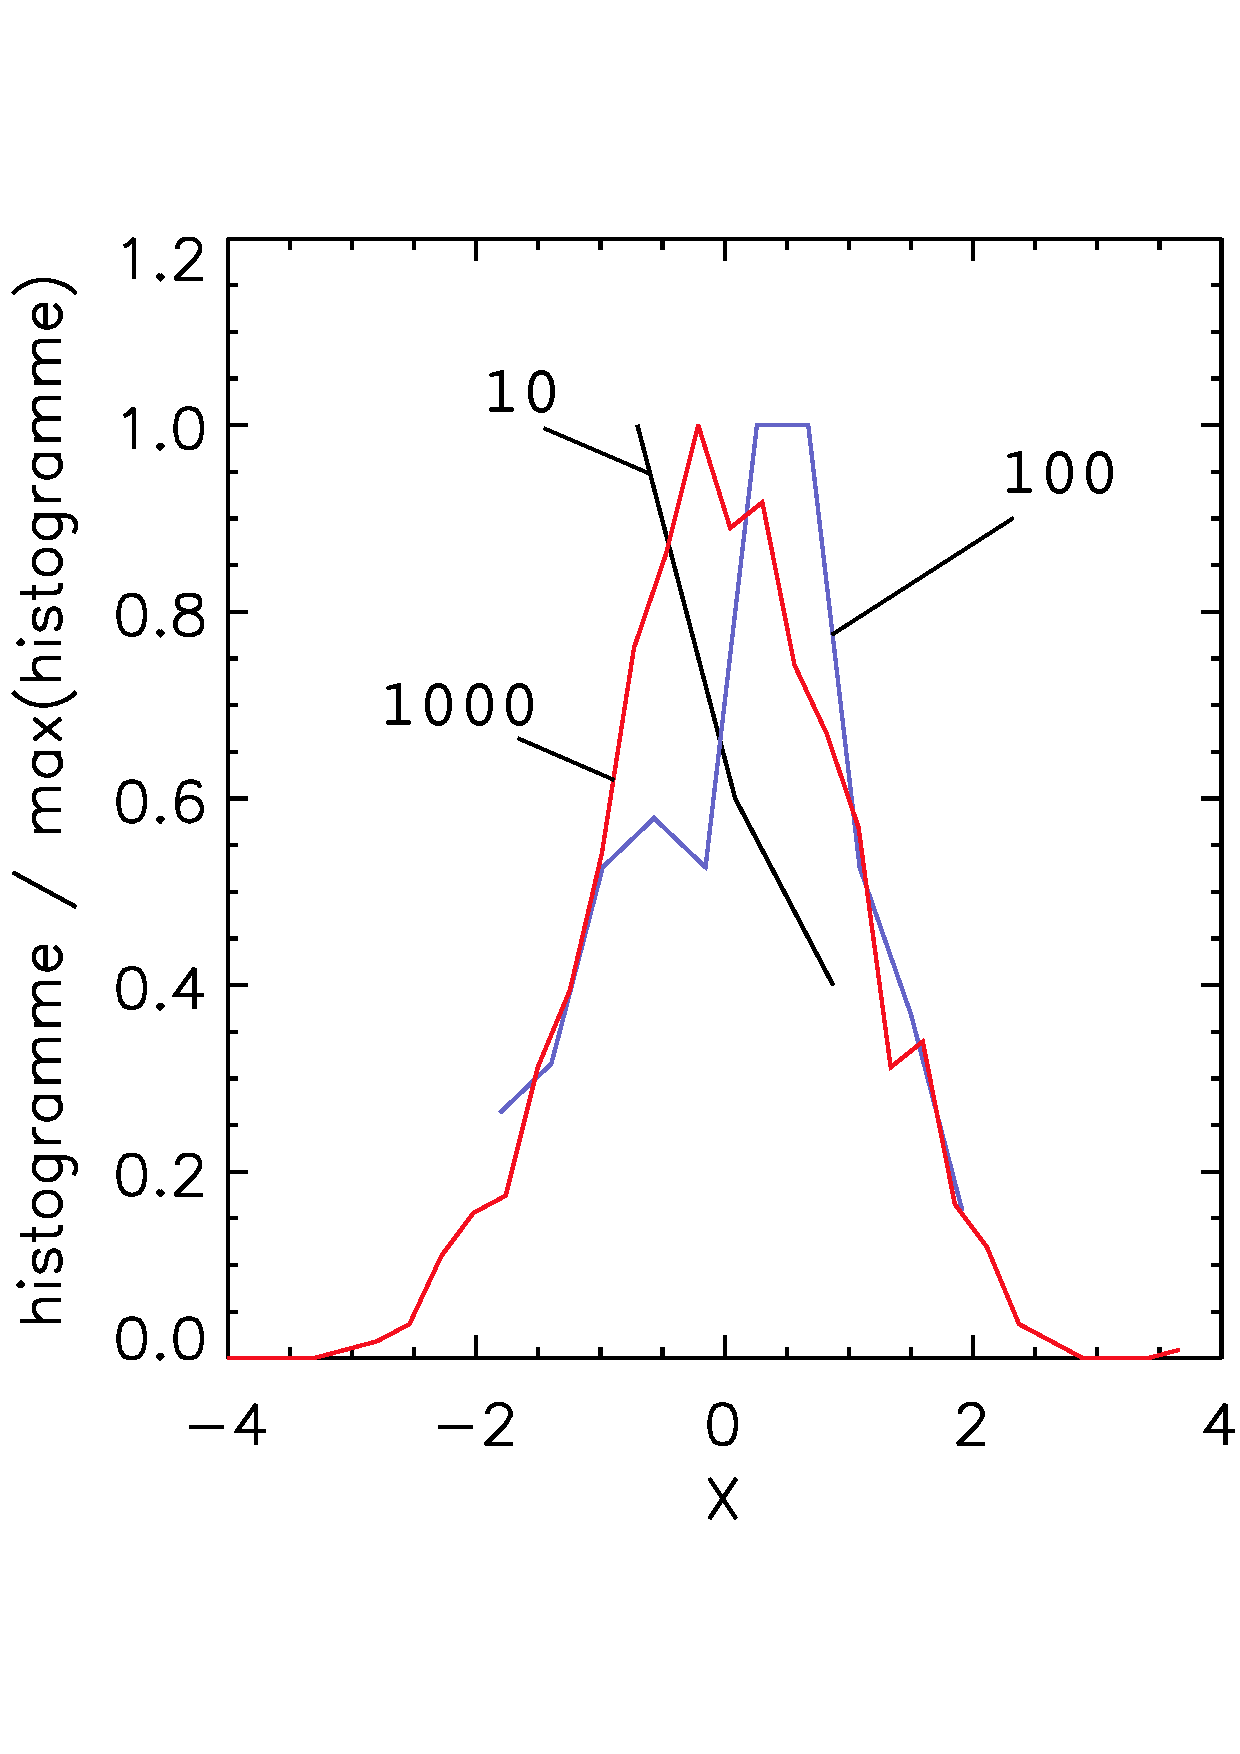
\includegraphics[width=6cm]{assets/figures/histGaussienDixCentMilleMesures.pdf}
   \caption{\it Histogramme d'une mesure gaussienne de moyenne nulle et d'écart-type 1, pour des échantillons de 10, 100 et 1000 mesures.}
   \label{fig:h123}
\end{wrapfigure}
distribution gaussienne, lorsque l'on considère 10, 100 et 1000 points de mesure. On voit qu'avec 10 points (et donc 3 classes), il est impossible de dire quoi que ce soit. Avec 100 points (courbe bleue, 10 classes) on commence à voir que la distribution est centrée, compacte, avec un maximum autour de 0. Avec 1000 points (30 classes), la distribution gaussienne devient évidente.

On peut montrer, en théorie statistique, que si on dispose de $N_m$ mesures d'une grandeur physique quelconque $G$, alors l'erreur commise sur la détermination de la vraie moyenne est égale à l'écart-type de l'échantillon divisé par la racine carrée de $N_m$,
\begin{equation}
\text{err}(\langle G\rangle)=\frac{\sigma_G}{\sqrt{N_m}}
\end{equation}
Par conséquent, l'erreur relative due au nombre fini de mesures va comme $1/\sqrt{N_m}$. Par conséquent, si on veut une précision de 1\% sur la moyenne, il faudra acquérir au moins 10'000 mesures. Cette règle fonctionne très bien, pour tout type de mesure.

\section{Histogramme cumulé}

Un autre outil de représentation pratique de l'échantillon est constitué par le cumul des fréquences, c.-à-d. la détermination du nombre de fois $F_k$ que la mesure x est comprise dans une classe donnée ou dans les classes précédentes,
$$
F_k=\text{nombre de fois que x $\in$ classes } 1,2,\cdots,k
$$
c.-à-d.
\begin{equation}
F_k=\sum\limits_{i=1}^{k}\,f_k
\end{equation}
\begin{wraptable}[6]{r}[0pt]{44mm}
\centering
\vspace{-6mm}
\begin{tabular}{cccccc}
 8 &  1 &  2 &  1 &  2 &  7 \\
 5 & 10 &  1 &  9 &  4 &  6 \\
10 &  9 &  5 &  4 &  2 &  3 \\
 5 &  2 &  0 &  1 &  5 &  4 \\
 4 &  6 &  6 &  7 &  4 &  5 \\
 6 &  4 & 10 &  3 &  0 &  4
\end{tabular}
\end{wraptable}
Considérons par exemple un échantillon de 36 éléments (ci-contre), tiré d'une distribution uniforme. La moyenne de l'échantillon est 4.72 et l'écart-type 3.00. Considérons 5 classes, et calculons les fréquences de chaque classe. La largeur des classes sera donnée par $\Delta x=(\text{max}(x)-\text{min}(x))/N_c=10/5=2$. On trouve
\begin{center}
\begin{tabular}{cccc}
classe $k$ & intervalle & val. centrale $x_k$ & fréquence $f_k$ \\\hline
1 & [0,2[ & 1 & 6 \\
2 & [2,4[ & 3 & 6 \\
3 & [4,6[ & 5 & 11 \\
4 & [6,8[ & 7 & 6 \\
5 & [8,10] & 9 & 7 \\\hline
\end{tabular}
\end{center}
L'histogramme correspondant est montré en Fig.~\ref{fig:hcapoabdc}, gauche. Les fréquences cumulées sont données ci-dessous, et l'histogramme cumulé correspondant en Fig.~\ref{fig:hcapoabdc}, droite.
\begin{center}
\begin{tabular}{ccccc}
classe $k$ & intervalle & val. centrale $x_k$ & fréquence $f_k$ & fréq. cum. $F_k$\\\hline
1 & [0,2[ & 1 & 6 & 6 \\
2 & [2,4[ & 3 & 6 & 12 \\
3 & [4,6[ & 5 & 11 & 23 \\
4 & [6,8[ & 7 & 6 & 29 \\
5 & [8,10] & 9 & 7 & 36\\\hline
\end{tabular}
\end{center}
\begin{figure}[h]
   \centering
   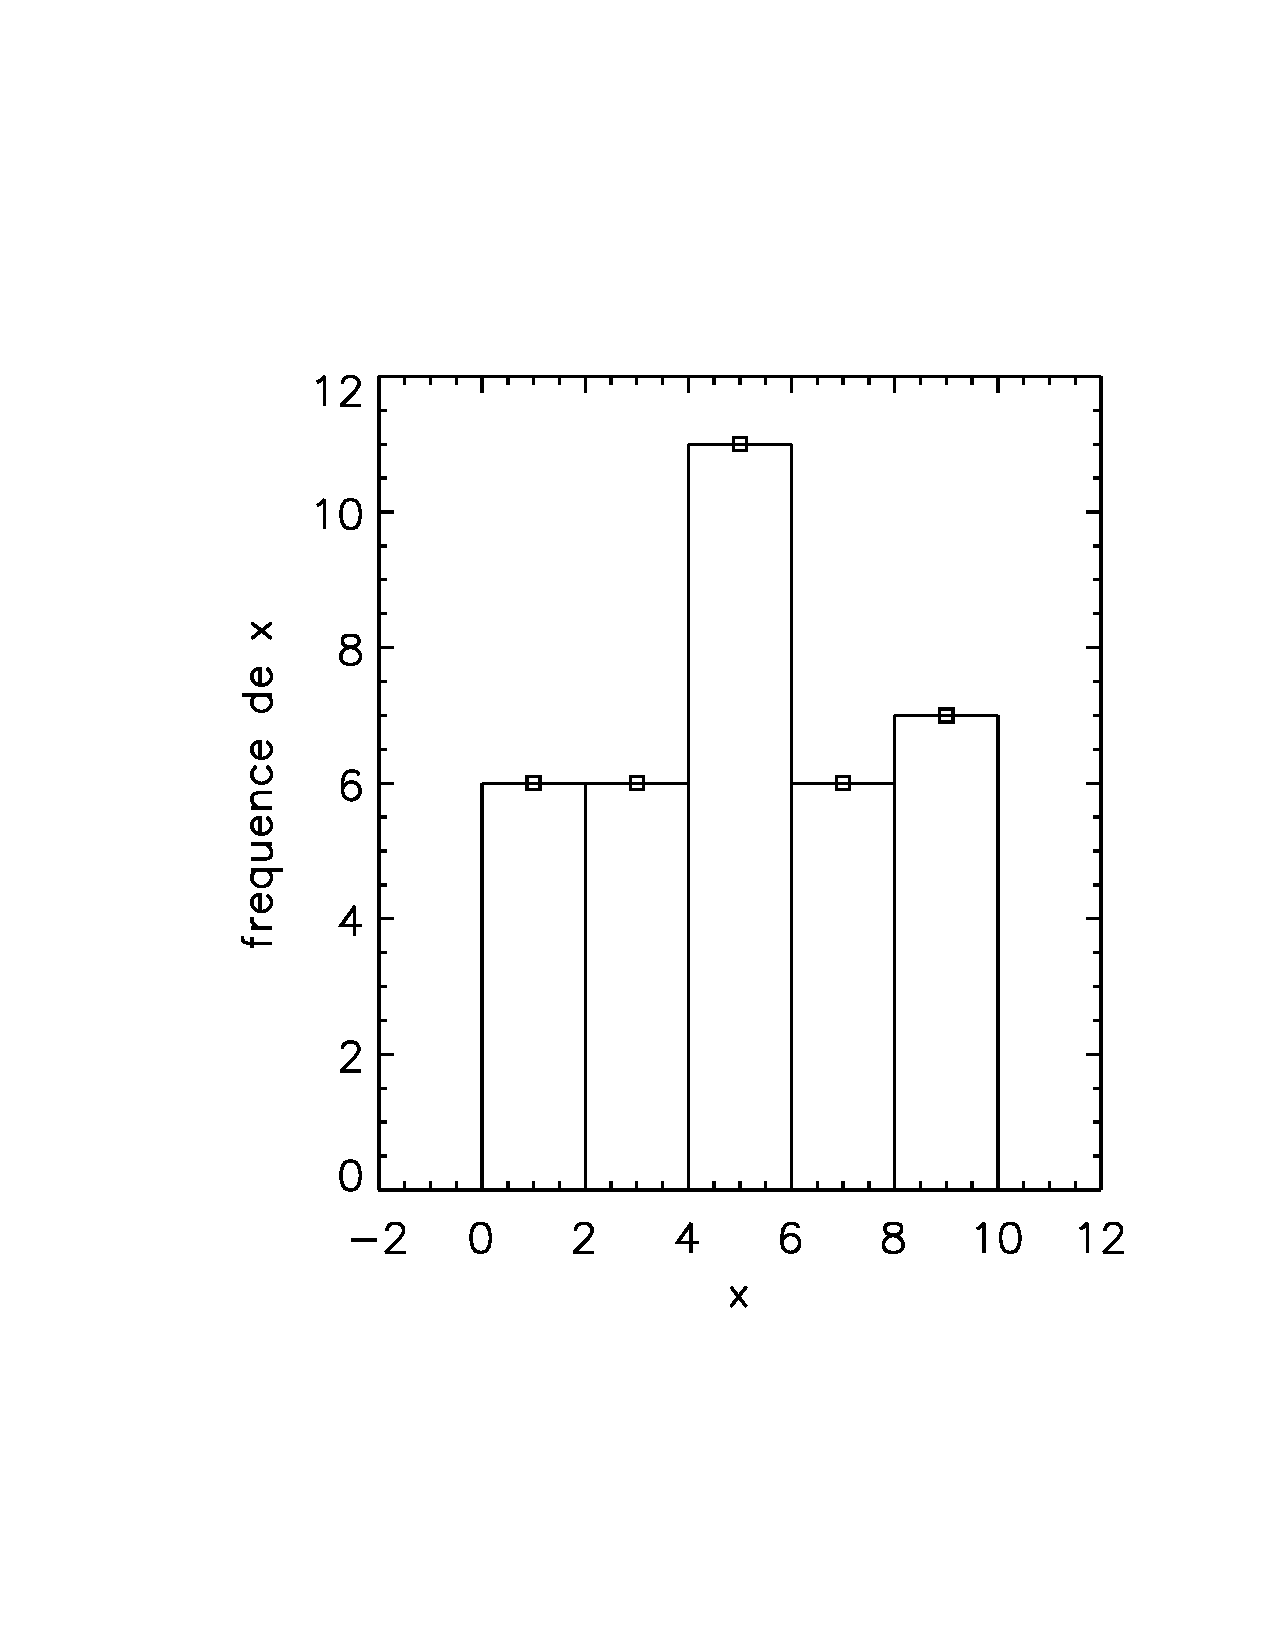
\includegraphics[width=5.5cm]{assets/figures/hist5classes.pdf}\hspace{5mm}
   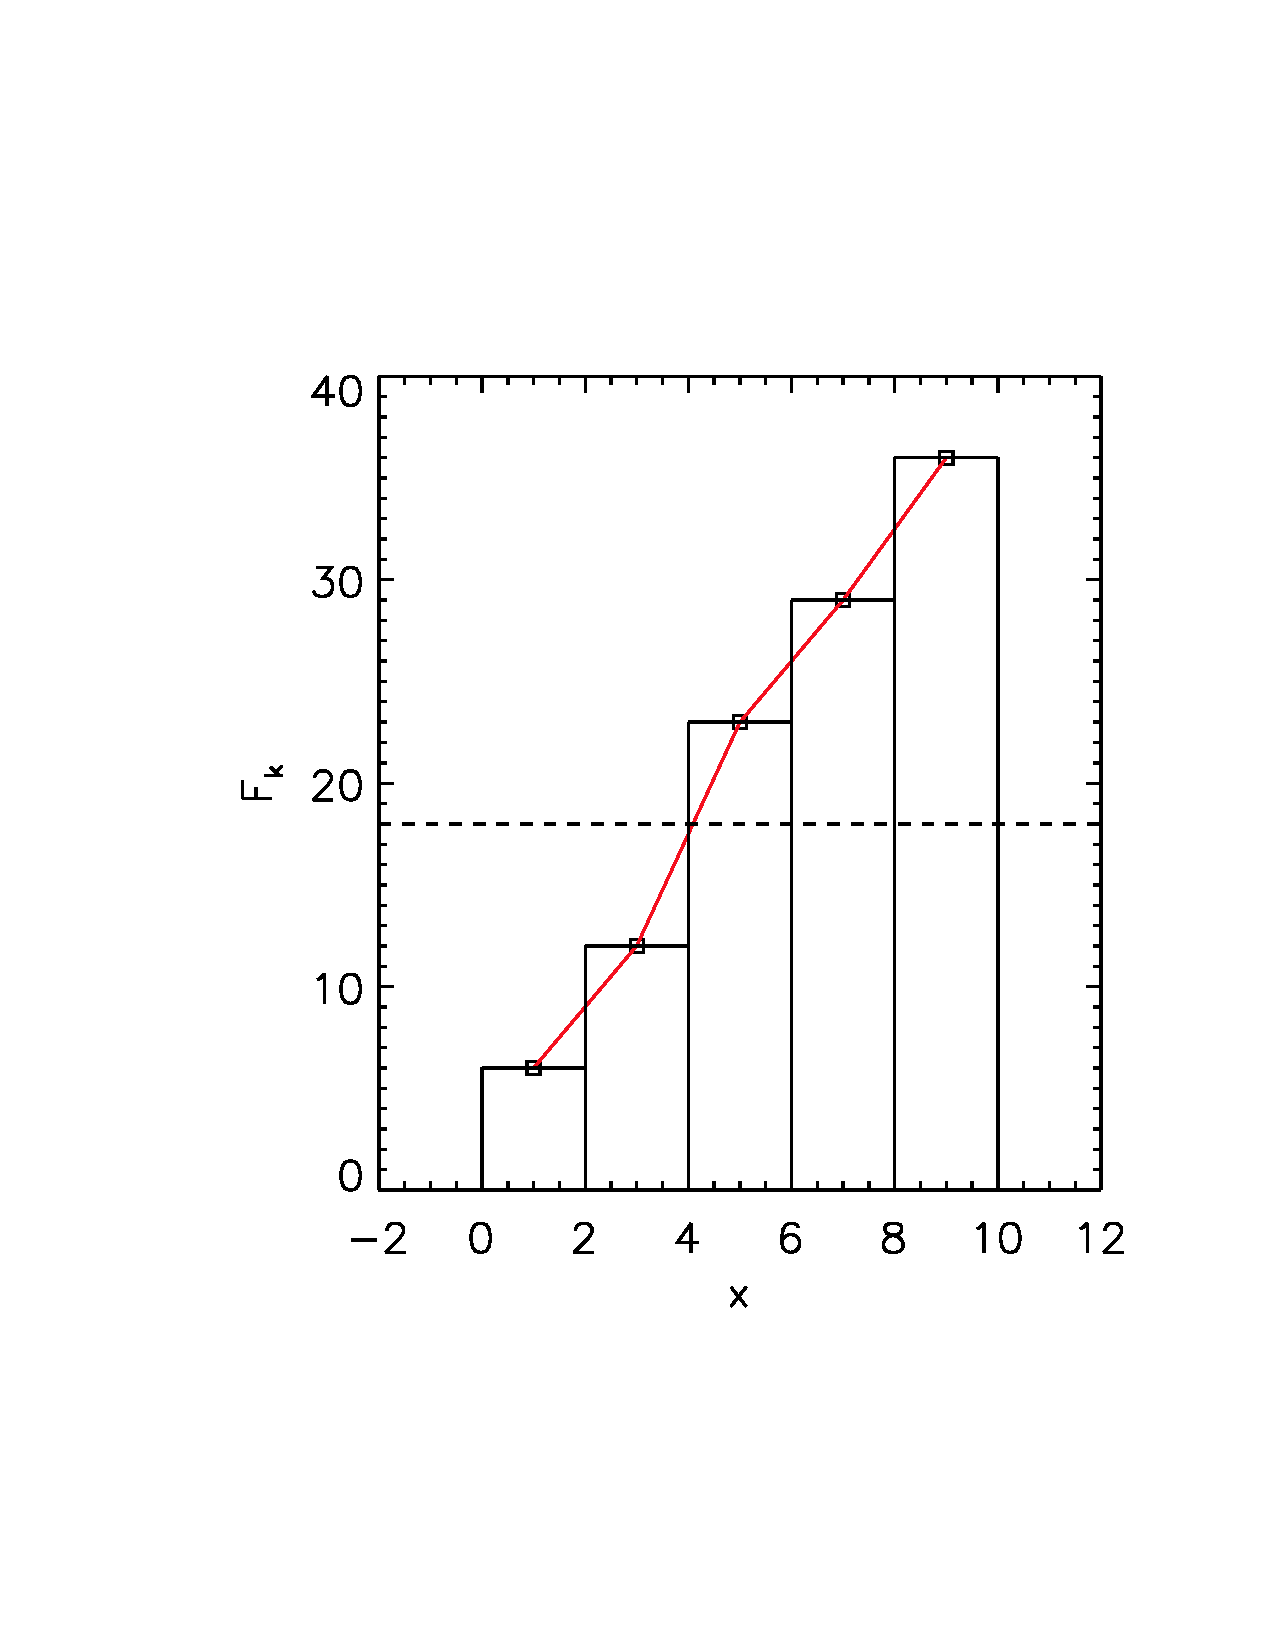
\includegraphics[width=5.5cm]{assets/figures/histCumul5classes.pdf}
   \caption{À gauche: histogramme des 36 mesures, pour 5 classes; à droite, histogramme cumulé correspondant. La ligne horizontale à la hauteur $N_m/2$ permet de repérer la médiane, ici égale à 4, par interpolation.}
   \label{fig:hcapoabdc}
\end{figure}
où on voit naturellement que $F_{N_c}=N_m$, c.-à-d. que la fréquence cumulée de la dernière classe est égale aux nombres de mesures. \textbf{L'histogramme cumulé} est simplement la représentation graphique de la fréquence cumulée. L'intérêt principal de l'histogramme cumulé est de mettre en évidence la valeur de la grandeur critique séparant les mesures en deux échantillons de dimension égale, \textbf{la médiane}, que nous introduisons ci-dessous.

Par ailleurs, puisque la fréquence cumulée est une somme, elle représente en quelque sorte l'intégrale de la fréquence; inversement, on peut interpréter la fréquence $f_k$ comme la dérivée de la fréquence cumulée. Nous reviendrons sur ces notions lors de l'introduction des distributions de probabilité, dans un prochain chapitre.

\section{Médiane et mode}

\subsection{Médiane}

La médiane de l'échantillon est définie par la valeur qui sépare l'histogramme des fréquences en deux parties de somme égales, en d'autres termes il existe autant de mesures de valeur inférieure à la médiane que de mesures de valeur supérieure à la médiane. La valeur médiane ne fait pas toujours partie de l'échantillon, ni de la population. Par exemple, dans l'exemple de l'échantillon à 36 mesures, il y a 12 valeurs inférieures ou égales à 3, mais 19 valeurs inférieures ou égales à 4. Or la médiane devrait séparer l'échantillon en 18 mesures inférieures à elle-même, et 18 mesures supérieures. Ce n'est pas possible avec cet échantillon. On choisira alors, pour la valeur médiane, la valeur partageant l'échantillon en deux parties de dimensions les plus égales possible, en l'occurrence, ici, 4.

À noter que lorsque l'histogramme est symétrique autour de la valeur moyenne, la médiane est naturellement égale à la moyenne de l'échantillon.

\subsection{Mode}

Le mode de l'échantillon est défini par la valeur la plus représentée, c'est-à-dire la valeur ayant la plus haute fréquence. Si l'échantillon consiste en une série de mesures ayant toutes des valeurs différentes, ce qui arrive souvent lorsque les mesures sont des nombres réels, alors la notion de mode n'a pas de sens, car aucune valeur n'est plus représentée qu'une autre.

En revanche, si on constitue l'histogramme de l'échantillon, et que l'on choisit un nombre de classes convenable (par exemple la racine carrée du nombre de mesures), alors le regroupement dans les classes va naturellement faire apparaitre une classe plus peuplée que les autres. La valeur associée sera alors le mode de l'échantillon.

Dans le cas de notre échantillon de 36 mesures, si les mesures sont réparties en 5 classes, on trouve alors que la classe numéro 3 est la plus représentée, correspondant aux mesures comprises dans l'intervalle 4 à 6.

\section{Exercices du chapitre 6}

\begin{center}
\Large \bf {\underline{Pour faire ces exercices, utilisez \texttt{matlab}}}
\end{center}

\subsection*{Exercice 6.1 - caractérisation de la qualité d'usinage de lentilles optiques}

Une industrie de matériel optique fabrique des lentilles de focale $f=100$ mm, plan-convexes (première surface plane, seconde surface sphérique). L'indice de réfraction du verre des lentilles est $n=1.5$. La relation entre la focale de la lentille et le rayon de courbure de la surface sphérique est
$$
f=\frac{R}{n-1}=2R
$$
Pour la mise au point du procédé de fabrication, 1000 lentilles sont usinées et leur rayon de courbure mesuré. Les 1000 mesures sont données - en mm - dans le fichier ASCII \texttt{RayonDeCourbure.txt} distribué avec cette série d'exercices. Chargez ces mesures au sein du logiciel de traitement de données \texttt{matlab}, et répondez aux questions suivantes:
\begin{enumerate}
\item on désire que la focale des lentilles soit égale à 100 mm avec une précision de 2\% (c.-à-d. que l'on accepte les lentilles dont la focale est dans l'intervalle 98-102 mm). Quelle est la proportion de bonnes lentilles dans notre échantillon ? Si on veut conserver 90\% des lentilles, quelle sera la précision de ces lentilles ?
\item calculez la moyenne, la médiane, le mode et l'écart-type de cet échantillon;
\item déterminez le coefficient d'asymétrie $\beta_1$ et d'aplatissement $\gamma_2$;
\item d'après la valeur de $\beta_1$ et de $\gamma_2$, à quelle forme d'histogramme vous attendez-vous ?
\item construisez la table de fréquences, puis l'histogramme, pour 5, 10, 20 et 40 classes;
\item vous devez présenter ces mesures à un collègue; quel nombre de classes vous semble le plus approprié ? (vous pouvez en choisir un autre nombre que ceux donnés ci-dessus);
\item votre collègue utilise le tableau des fréquences que vous lui avez présenté pour calculer la moyenne et l'écart-type de l'échantillon, et arrive à des chiffres différents de ce que vous avez calculé au premier point ci-dessus. Expliquez-lui pourquoi ce sont vos résultats qui sont les bons.
\end{enumerate}

\subsection*{Exercice 6.2 - distance de pénétration des rayons $\gamma$ dans un substrat de germanium}

On dispose de 50 mesures de la distance de pénétration en mm (avant absorption) de photons $\gamma$ (rayons gamma à très haute énergie) dans un morceau de germanium,
\begin{center}
\begin{tabular}{|r|r|r|r|r|r|r|r|r|r|}
3088 & 1749 & 4085 & 1906 & 782 & 3683 & 1706 & 6445 & 2431 & 1418 \\
3544 & 1398 & 625 & 2094 & 3807 & 1617 & 969 & 810 & 748 & 1535 \\
5014 & 2255 & 4899 & 1726 & 1552 & 1811 & 524 & 980 & 41 & 2068 \\
386 & 4084 & 615 & 388 & 1955 & 989 & 2206 & 6407 & 1019 & 1180 \\
1448 & 673 & 4029 & 6589 & 2434 & 4388 & 2955 & 2010 & 1709 & 1064
\end{tabular}
\end{center}
Ces données sont contenues dans le fichier \texttt{PhotonsGammaGermanium.txt} distribué avec cette série d'exercices. Lancez \texttt{matlab} et chargez cette série dans une variable.
\begin{enumerate}
\item Calculez la moyenne, la médiane, le mode et l'écart-type de cet échantillon;
\item déterminez le coefficient d'asymétrie $\beta_1$ et d'aplatissement $\gamma_2$;
\item d'après la valeur de $\beta_1$ et de $\gamma_2$, à quelle forme d'histogramme vous attendez-vous ?
\item construisez la table de fréquences, puis l'histogramme, pour des classes de 300 mm, 1200 mm et 3000 mm de large, à l'aide d'un programme \texttt{matlab};
\item calculez la moyenne et l'écart-type à partir des tables de fréquences, avec et sans la correction de Sheppard;
\item calculez la médiane et le mode pour l'histogramme de largeur de classe 1200 mm.
\end{enumerate}

\subsection*{Exercice 6.3 - mesure de la pression atmosphérique martienne, Gusev crater, Mars}

Le robot d'exploration Curiosity a mesuré, le 17 novembre 2014, la pression atmosphérique à 1 m du sol, en pascal (Pa). 275 points de mesure ont étés enregistrés. Les mesures sont données dans le fichier \texttt{GroundPressureGusev.txt} distribué avec cette série d'exercices. Chargez ces mesures au sein de \texttt{matlab}, et répondez aux questions suivantes:
\begin{enumerate}
\item choisir un nombre de classes tel qu'il y a au moins 10 mesures dans la classe la plus peuplée;
\item calculez le tableau des fréquences cumulées;
\item représentez l'histogramme cumulé correspondant;
\item afin que l'eau puisse rester liquide au sol, à $10^{\circ}$C, il faut que la pression soit supérieure à 890 Pa; quelle est alors la probabilité que l'eau puisse rester liquide pendant les phases de haute pression ?
\end{enumerate}

%\end{document}